\chapter{Conception g\'enerale du projet}

\section{Introduction}
Ce chapitre est consacr\'e \`a la conception g\'en\'erale du projet. Apr\`es la d\'efinition des besoins fonctionnels et non fonctionnels, nous allons passer \`a la conception de l'architecture fonctionnelle qui repr\'esente une vue globale de la solution avec une prise en consid\'eration du besoin de la modularit\'e. 

\section{Conception g\'en\'erale}


\subsection{Architecture globale du syst\`eme}

Apr\`es la d\'efinition des besoins fonctionnels et non fonctionnels, nous avons pass\'e \`a la conception de l'architecture fonctionnelle qui repr\'esente une vue globale de la solution avec une prise en consid\'eration du besoin de la modularit\'e. Comme le montre la figure suivante :

\begin{figure}[H]
	\center{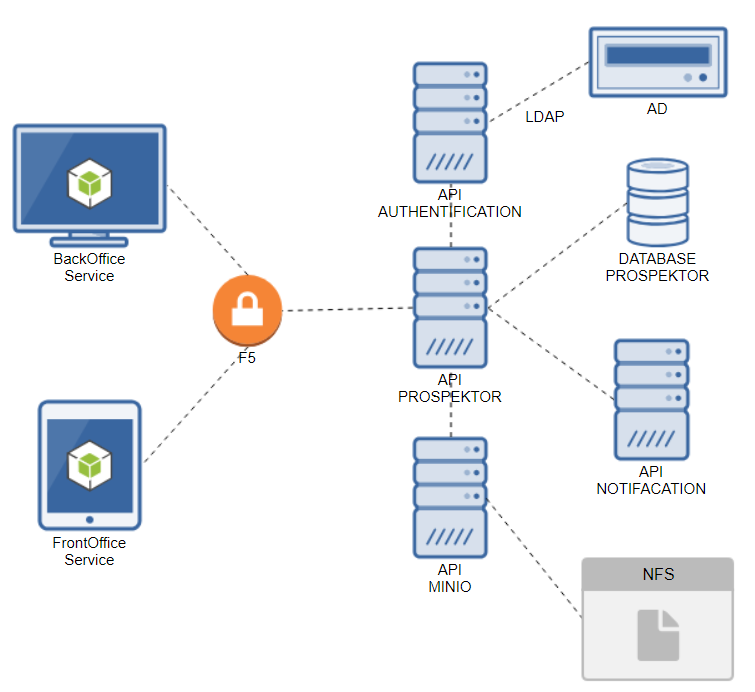
\includegraphics[width=0.55\textwidth]{Figures/architecture.PNG}}
	\caption{\label{fig:my-label} Architecture du syst\`eme}
\end{figure}

Cette architecture est d\'efinie pour les prospecteurs et les exploitant qui vont utiliser notre application mobile.

architecture du syst\`eme est compose par:
\begin{itemize}
\item \textbf{F5 VPN} : utilise le protocole Secure Sockets Layer, une technologie d'authentification et de cryptage int\'egr\'ee \`a chaque navigateur Web, pour cr\'eer une connexion s\'ecuris\'ee et crypt\'ee sur un r\'eseau moins s\'ecuris\'e, comme Internet.
\end{itemize}

